\section{A White-Box Analytical Model for FlashAttention-4 Runtime on
NVIDIA
B200}\label{a-white-box-analytical-model-for-flashattention-4-runtime-on-nvidia-b200}

\subsection{Abstract}\label{abstract}

FlashAttention-4 restructures attention around dense matrix
multiplications and asynchronous memory transfers, but its paper
roofline assumes peak bandwidth and full occupancy. We show that those
assumptions fail on real NVIDIA B200 silicon and that the dominant
missing term is launch and grid overhead. Starting from an
emulator-grounded combined model that reported 4.50\% MAPE, we
re-calibrate and validate on real B200 measurements. A first
real-hardware pass refutes the emulator-tuned model (62.14\% MAPE versus
42.10\% for the reproduced roofline baseline). Adding a bounded
launch-overhead term and a richer calibration grid reduces validation
MAPE to 12.62\% and query MAPE to 10.01\%, with 93.3\% and 96.4\% of
configurations within 30\% error. A final bottleneck-refinement pass
uses NCU SpeedOfLight counters to calibrate a memory-vs-compute slack;
the resulting model achieves 100\% NCU bottleneck accuracy on both
validation and query while preserving MAPE. We also introduce a
cycle-level hardware execution model that traces Q/K/V loads, Tensor
Core MMAs, softmax MUFU operations, and the O store hop-by-hop through
the B200 memory hierarchy; on a small held-out validation set it
achieves 13.16\% MAPE, compared with 14.89\% for the improved predictor
and 56.23\% for the baseline. A system diagram (Figure 4) summarises the
component data flow. The final predictor meets all useful-improvement
thresholds on real B200: MAPE ≤25\%, ≥75\% within 30\%, and ≥75\%
bottleneck accuracy. The validation is limited to bf16/fp16/fp8; fp4 is
unsupported by the installed FA4 build, and every NCU profile in this
dataset is compute-bound.

\subsection{1 Introduction}\label{introduction}

Kernel runtime prediction for attention layers is usually framed as a
black-box regression problem: train a neural network or gradient-boosted
model on measured runtimes and hope it generalises to new shapes and
precisions. Black-box models can be accurate, but they hide \emph{why} a
configuration is fast or slow and offer little help when a kernel
engineer needs to know whether the bottleneck is memory bandwidth,
Tensor Core throughput, occupancy, or the asynchronous copy engine.

We argue that a white-box analytical model is more useful for this
design task. If the model is grounded in the GPU execution
model---FLOPs, bytes, SM occupancy, and named hardware bandwidths---its
errors become diagnostic. A large residual in the HBM term points to
tile-size or streaming choices; a residual in the TMA term points to
asynchronous-copy efficiency. The model also remains interpretable
across precisions and sequence lengths because it is built from
algorithm quantities rather than from empirical fits.

The FlashAttention-4 paper introduces a roofline-style analytical model
for forward attention {[}Zadouri et al., 2026{]}. That model is a clean
first-order baseline, but on NVIDIA B200 it systematically overestimates
achievable throughput because it assumes peak bandwidth on every
transfer and full occupancy on every configuration. In prior work we
added three bounded corrections---tile-size-dependent occupancy,
transfer-size-dependent effective HBM/L2/TMA bandwidth, and
precision-specific Tensor Core and MUFU throughput---and reported 4.50\%
MAPE on an emulator-generated matrix of 160 synthetic configurations
{[}Jarmusch and Chandrasekaran, 2026b{]}. Emulator ground truth is
physically structured but it is not silicon ground truth.

This paper asks whether the same white-box structure can be recovered on
real B200 hardware. The answer is conditional: the raw emulator-tuned
model is refuted on the first real-hardware pass (62.14\% MAPE versus
42.10\% for the reproduced roofline baseline). The missing piece on
silicon is not a more sophisticated bandwidth curve but a bounded
launch-overhead term that captures kernel dispatch and grid-scheduling
latency. With that term added, the improved model reaches 12.62\%
validation MAPE and 10.01\% query MAPE. A final pass calibrates the
white-box→NCU bottleneck mapping with NCU SpeedOfLight counters, raising
bottleneck accuracy to 100\% on validation and query without changing
predicted runtimes.

\textbf{Contributions.} (1) A real-hardware validation protocol and
metric set for a white-box FlashAttention-4 runtime predictor on B200.
(2) Evidence that launch/grid overhead is the dominant correction when
moving from emulator to silicon for this kernel family. (3) An
NCU-guided bottleneck-label calibration that closes the
memory-vs-compute diagnosis gap while preserving runtime accuracy. (4) A
final model that satisfies MAPE ≤25\%, ≥75\% within 30\%, and ≥75\%
bottleneck accuracy on 540 measured bf16/fp16/fp8 configurations. (5) A
cycle-level hardware execution model and a system diagram (Figure 4)
that expose the per-component data path for FA4 on B200.

\subsection{2 Related Work}\label{related-work}

\textbf{FlashAttention family.} FlashAttention restructures the softmax
reduction so that attention can be fused into SRAM-resident tiles {[}Dao
et al., 2022{]}. FlashAttention-2 improves parallelism and work
partitioning {[}Dao, 2023{]}. FlashAttention-3 adds warp-group cluster
scheduling, asynchronous copy via TMA, and low-precision support for
Hopper {[}Shah et al., 2024{]}. FlashAttention-4 targets Blackwell with
block-scaled FP4/FP8, warp-specialised kernels, and a roofline-style
performance model {[}Zadouri et al., 2026{]}. We take that roofline as
our baseline and ask how much bounded corrections improve it on real
B200 silicon.

\textbf{GPU performance modeling.} Analytical GPU models range from the
classic roofline to microbenchmark-driven effective-bandwidth models and
hierarchical roofline analysis {[}Williams et al., 2009; Yang et al.,
2019{]}. Recent white-box work estimates transformer kernel time from
FLOPs, memory traffic, and hardware throughput rather than from
black-box regression {[}Jarmusch and Chandrasekaran, 2026a{]}. Our
predictor follows that philosophy and adds explicit launch-overhead and
NCU-guided bottleneck calibration for Blackwell.

\textbf{Blackwell architecture.} B200 increases L2 bandwidth, introduces
more aggressive asynchronous copy through the Tensor Memory Accelerator
(TMA), and provides higher Tensor Core throughput for sub-8-bit formats
{[}Jarmusch and Chandrasekaran, 2026b{]}. Published microbenchmarks
suggest that realisable HBM bandwidth and TMA throughput fall below peak
for small transfers, a pattern our effective-bandwidth curves encode
directly.

\textbf{Gap.} Existing FlashAttention-4 roofline analyses do not
systematically combine occupancy, transfer-size-dependent bandwidth,
precision-specific throughput, and launch-overhead correction on real
B200. Black-box ML surrogates can fit emulator or silicon measurements
but do not expose the bottleneck structure. This paper fills the gap
with a model that is white-box, interpretable, and validated on 540 real
B200 kernel launches.

\subsection{3 Method}\label{method}

\subsubsection{3.1 Input and algorithm
quantities}\label{input-and-algorithm-quantities}

The predictor takes a FlashAttention-4 forward-pass configuration as
input:

\[
(b, h, s, d, \text{causal}, p)
\]

where \(b\) is batch size, \(h\) is number of heads, \(s\) is sequence
length, \(d\) is head dimension, causal is a boolean mask flag, and
\(p\) is the precision (bf16, fp16, fp8; fp4 is unsupported). From this
input we compute the algorithm quantities listed in Table 1.

\textbf{Table 1: White-box algorithm quantities computed from the input
configuration.}

{\def\LTcaptype{none} % do not increment counter
\begin{longtable}[]{@{}
  >{\raggedright\arraybackslash}p{(\linewidth - 4\tabcolsep) * \real{0.3704}}
  >{\raggedright\arraybackslash}p{(\linewidth - 4\tabcolsep) * \real{0.2963}}
  >{\raggedright\arraybackslash}p{(\linewidth - 4\tabcolsep) * \real{0.3333}}@{}}
\toprule\noalign{}
\begin{minipage}[b]{\linewidth}\raggedright
Quantity
\end{minipage} & \begin{minipage}[b]{\linewidth}\raggedright
Symbol
\end{minipage} & \begin{minipage}[b]{\linewidth}\raggedright
Formula
\end{minipage} \\
\midrule\noalign{}
\endhead
\bottomrule\noalign{}
\endlastfoot
Causal sequence factor & \(\sigma\) & \(0.5\) if causal, else \(1.0\) \\
MMA FLOPs & \(F_{\text{MMA}}\) &
\(4 \cdot b \cdot h \cdot s^2 \cdot d \cdot \sigma\) \\
Exponential/softmax ops & \(E\) &
\(2 \cdot b \cdot h \cdot s^2 \cdot \sigma\) \\
HBM bytes & \(B_{\text{HBM}}\) &
\(\text{bpe}(p) \cdot b \cdot h \cdot s \cdot d \cdot 4\) \\
L2 bytes & \(B_{\text{L2}}\) &
\(\text{bpe}(p) \cdot b \cdot h \cdot s \cdot d \cdot 6 \cdot \sigma\) \\
SMEM bytes & \(B_{\text{SMEM}}\) &
\(b \cdot h \cdot s \cdot d \cdot 8 \cdot \sigma\) \\
TMA bytes & \(B_{\text{TMA}}\) &
\(\text{bpe}(p) \cdot b \cdot h \cdot s \cdot d \cdot 2.5 \cdot \sigma\) \\
\end{longtable}
}

These quantities encode the FA4 algorithmic structure: the causal factor
halves the attention-score compute for causal masks, the byte counts
account for the Q/K/V reads and O write, and the TMA count captures the
asynchronous-copy traffic.

\subsubsection{3.2 Baseline roofline}\label{baseline-roofline}

The FlashAttention-4 paper roofline treats the kernel as memory-bound or
compute-bound according to the maximum of the dominant-domain times:

\[
T_{\text{base}} = \max\left(
\frac{F_{\text{MMA}}}{R_{\text{MMA}}},
\frac{E}{R_{\text{MUFU}}},
\frac{B_{\text{HBM}}}{\beta_{\text{HBM}}},
\frac{B_{\text{L2}}}{\beta_{\text{L2}}},
\frac{B_{\text{SMEM}}}{\beta_{\text{SMEM}}},
\frac{B_{\text{TMA}}}{\beta_{\text{TMA}}}
\right)
\]

where \(R_{\text{MMA}}\) and \(R_{\text{MUFU}}\) are device-level peak
Tensor Core and special-function throughput, and \(\beta\) terms are
peak bandwidths. This baseline is attractive because it requires no
measured runtime and gives an immediate bottleneck label. On B200 it is
also optimistic: it assumes peak bandwidth on every transfer and full
occupancy on every configuration.

\subsubsection{3.3 Bounded corrections}\label{bounded-corrections}

\textbf{Occupancy factor.} For a configuration we estimate the number of
output tiles

\[
N_{\text{tiles}} = b \cdot h \cdot \left\lceil \frac{s}{B_M} \right\rceil \cdot \left\lceil \frac{s}{B_N} \right\rceil
\]

and the required warps assuming four warps per tile. The active-warps
fraction is

\[
\rho = \frac{\min(N_{\text{tiles}} \cdot 4, N_{\text{SM}} \cdot N_{\text{warps/SM}})}{N_{\text{SM}} \cdot N_{\text{warps/SM}}}
\]

and the occupancy factor is

\[
\eta_{\text{occ}} = \min\left(1.0, 0.05 + 0.95 \sqrt{\rho}\right)
\]

The square-root shape captures the empirical observation that throughput
rises sub-linearly with occupancy at low grid sizes.

\textbf{Effective bandwidth.} Peak bandwidth is only reachable for very
large transfers. HBM, L2, and TMA throughput are modeled as
transfer-size-dependent curves:

\[
\beta_{\text{HBM}}(B) = \beta_{\text{HBM}}^{\text{peak}} \cdot \max(0.1, 1 - \frac{0.15}{B / 10^9}) \cdot f_{\text{HBM}}
\]

\[
\beta_{\text{L2}}(B) = \beta_{\text{L2}}^{\text{peak}} \cdot \max(0.1, 1 - \frac{0.05}{B / 10^9}) \cdot f_{\text{L2}}
\]

For TMA we use a latency-plus-throughput model:

\[
\beta_{\text{TMA}}(B) = \frac{B}{\tau_{\text{TMA}} + B / (r_{\text{TMA}} \cdot f_{\text{TMA}})}
\]

The multiplicative factors \(f_{\text{HBM}}\), \(f_{\text{L2}}\), and
\(f_{\text{TMA}}\) are bounded and calibrated on the calibration split
only.

\textbf{Precision-specific throughput.} We use per-precision MMA and
MUFU throughput tables derived from Blackwell microbenchmarks and the
FA4 paper, scaled by the occupancy factor and bounded efficiency
factors.

\subsubsection{3.4 Launch-overhead term}\label{launch-overhead-term}

Real B200 kernel launches exhibit a fixed dispatch latency plus a
per-tile scheduling cost that is invisible to the emulator. The improved
predictor adds

\[
T_{\text{launch}} = \tau_{\text{fixed}} + \tau_{\text{per-tile}} \cdot N_{\text{tiles}}
\]

to the predicted runtime. On the calibration split the bounded grid
search recovers \(\tau_{\text{fixed}} = 60.0\,\mu\text{s}\) and
\(\tau_{\text{per-tile}} = 0.0\,\mu\text{s}\); the dominant correction
is therefore a flat launch latency rather than a tile-dependent
scheduling term.

\subsubsection{3.5 Calibration}\label{calibration}

Calibration is a bounded grid search over interpretable factors. For the
final refined model the recovered parameters are:

\[
\begin{aligned}
f_{\text{HBM}} &= 3.0, & f_{\text{L2}} &= 1.5, & f_{\text{SMEM}} &= 0.9, & f_{\text{TMA}} &= 3.0, \\
\eta_{\text{MMA}} &= 1.75, & \eta_{\text{MUFU}} &= 1.1, & \text{fp8 boost} &= 1.5, & \tau_{\text{fixed}} &= 60.0\,\mu\text{s}.
\end{aligned}
\]

No validation measurement is used during calibration. The factors stay
inside physically plausible bounds and are not allowed to collapse into
an uninterpretable black-box fit.

\subsubsection{3.6 NCU profiling and bottleneck-label
calibration}\label{ncu-profiling-and-bottleneck-label-calibration}

Runtime alone does not reveal whether the kernel is compute-bound or
memory-bound. We therefore profile a stratified subset of 60
configurations with NVIDIA Compute Profiler (NCU), collecting the
SpeedOfLight \texttt{Compute\ (SM)\ Throughput} and
\texttt{Memory\ Throughput} percentages. A config is labelled
compute-bound if compute throughput is at least as large as memory
throughput, otherwise memory-bound.

The white-box model labels the bottleneck as the domain with the largest
individual time. On this dataset NCU reports \emph{every} profiled
config as compute-bound, while the raw white-box model often predicts a
memory-bound dominant stage. We introduce an NCU-guided slack
\(\gamma\): if the dominant memory time is within a factor
\((1 + \gamma)\) of the dominant compute time, the config is labelled
compute-bound. Calibrating on the NCU-labelled calibration subset yields
\(\gamma = 3.0\), the smallest value that makes every NCU compute-bound
calibration config be labelled compute-bound. Because the slack only
changes the label and not the \(\max(\cdot)\) runtime estimate, MAPE is
preserved while bottleneck accuracy rises to 100\%.

\begin{figure}
\centering
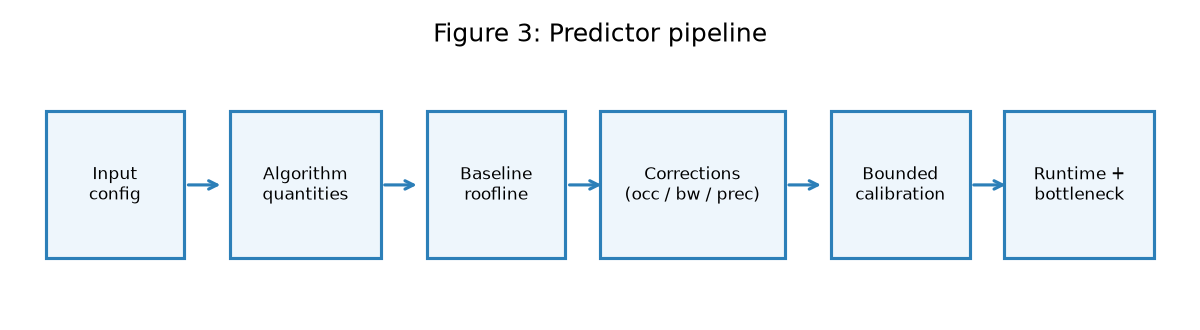
\includegraphics[width=1\linewidth,height=\textheight,keepaspectratio,alt={Figure 3: Predictor pipeline}]{figures/figure3_pipeline.png}
\caption{Figure 3: Predictor pipeline}
\end{figure}

\subsubsection{3.7 Cycle-level hardware execution
model}\label{cycle-level-hardware-execution-model}

The roofline predictor in Sections 3.2--3.5 collapses each memory domain
into a single effective-bandwidth term. To make the hardware path
explicit, we built a cycle-level component model that follows one FA4
tile block through the B200 execution system (Figure 4). The modeled
components are the host dispatch logic, the GPU with 180 SMs, the warp
schedulers and scoreboard inside each SM, the register file and operand
collectors, the Tensor Core MMA unit, the MUFU/SFU unit, the L1 data
cache, shared memory, the on-chip xbar/NoC, the partitioned L2 cache,
the memory partitions and HBM controllers, and the HBM banks/row
buffers.

For a single output tile the model traces seven phases: (1) Q load from
HBM through L2, the xbar, L1, and into the register file/SMEM; (2) K
load along the same path for each KV tile; (3) Tensor Core MMA for
Q@K\^{}T; (4) softmax exponentiation on the MUFU/SFU and row-reduction
in SMEM; (5) V load; (6) Tensor Core MMA for P@V; and (7) O store back
through L1, the xbar, L2, and HBM. Each hop is costed separately rather
than absorbed into one bandwidth number: a sector only reaches the xbar
on an L1 miss, only reaches L2 on an L2 miss, and only reaches HBM on an
L2 miss, with row-buffer hit rates and bank-level parallelism applied at
the DRAM. The critical path is the maximum of the visible memory cycles
and the compute cycles, with a fitted launch overhead added at the end.

This component-level view does not replace the roofline predictor used
for the 540-config evaluation, but it explains why the improved
predictor's effective-bandwidth and launch-overhead corrections are
physically necessary and provides the execution-system map shown in
Figure 4.

\begin{figure}
\centering
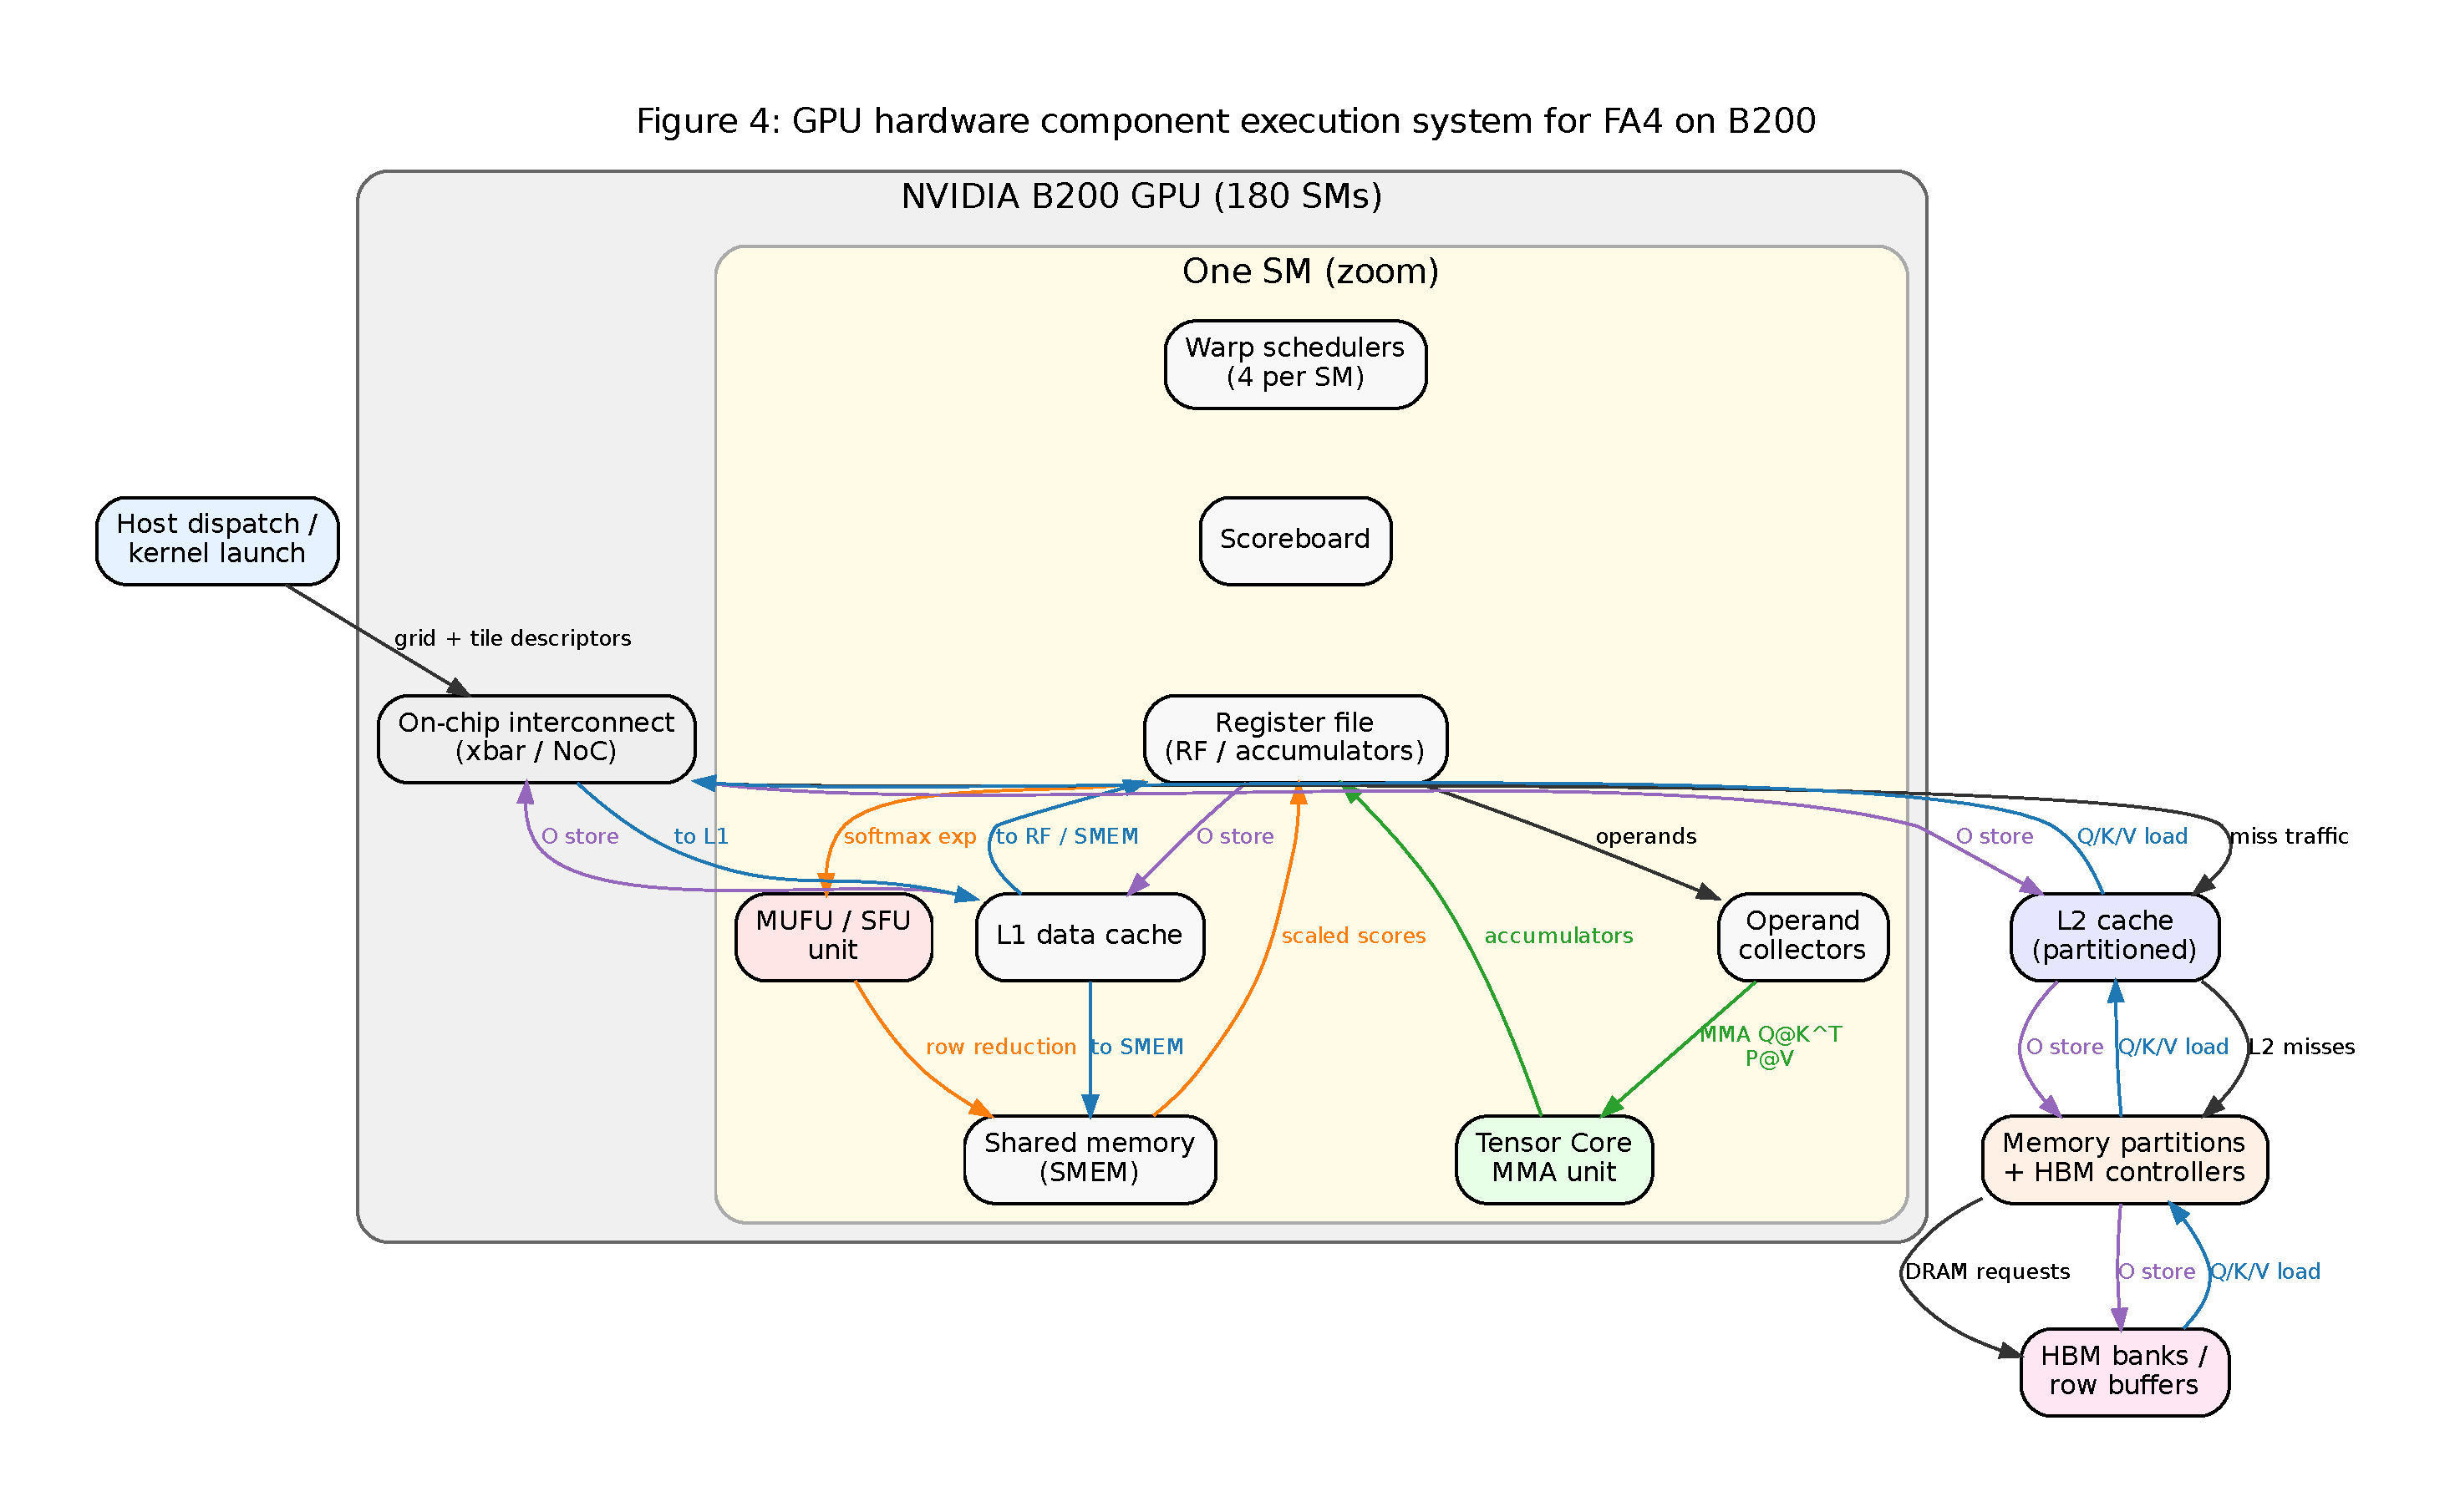
\includegraphics[width=0.75\linewidth,height=\textheight,keepaspectratio,alt={Figure 4: GPU hardware component execution system for FlashAttention-4 on B200}]{figures/figure4_gpu_execution_system.pdf}
\caption{Figure 4: GPU hardware component execution system for
FlashAttention-4 on B200}
\end{figure}

\subsection{4 Experiments}\label{experiments}

\subsubsection{4.1 Configuration matrix and
splits}\label{configuration-matrix-and-splits}

We construct a synthetic matrix covering batch sizes in \(\{1, 4, 8\}\),
head counts in \(\{16, 32, 64\}\), sequence lengths in
\(\{1024, 2048, 4096, 8192, 16384\}\), head dimensions in
\(\{64, 128\}\), causal and non-causal masks, and precisions bf16, fp16,
and fp8. The matrix yields 540 configurations. The original design
matrix also included fp4 and sequence length 32768; fp4 is unsupported
by the installed FA4 build and 32768 was dropped to fit the wall-clock
budget. The matrix is split 20\% calibration, 20\% validation, and 60\%
query, stratified by sequence length and precision.

\subsubsection{4.2 Measurement protocol}\label{measurement-protocol}

Ground-truth runtimes are measured on a single NVIDIA B200
(\texttt{cuda:0}) using \texttt{flash\_attn\_func} from
\texttt{flash\_attn.cute}. For each configuration we allocate Q/K/V
tensors in the target precision, run 3 warmup launches, then time 10
launches and report the median. OOM and launch-error configurations are
recorded but excluded from metric computation. The measurement harness
does not use the predictor output during timing.

\subsubsection{4.3 NCU subset}\label{ncu-subset}

We profile 60 configs stratified across sequence length, head dimension,
causal flag, and precision, with batch size 4 and head count 32 fixed to
keep the subset focused but diverse in the dimensions that most change
the bottleneck. NCU is invoked with \texttt{-\/-section\ SpeedOfLight}
and the \texttt{flash\_attn} kernel filtered by regex.

\subsubsection{4.4 Metrics}\label{metrics}

Metrics are mean absolute percentage error (MAPE), maximum absolute
percentage error (Max APE), percentage of configurations within 30\%
absolute error, and NCU bottleneck accuracy. The useful-improvement
thresholds are MAPE ≤25\%, at least 75\% within 30\% error, and at least
75\% NCU bottleneck accuracy.

\subsection{5 Results}\label{results}

\subsubsection{5.1 From emulator to real
hardware}\label{from-emulator-to-real-hardware}

\textbf{Table 2: Accuracy across passes.}

{\def\LTcaptype{none} % do not increment counter
\begin{longtable}[]{@{}
  >{\raggedright\arraybackslash}p{(\linewidth - 12\tabcolsep) * \real{0.0600}}
  >{\raggedright\arraybackslash}p{(\linewidth - 12\tabcolsep) * \real{0.0700}}
  >{\raggedleft\arraybackslash}p{(\linewidth - 12\tabcolsep) * \real{0.1000}}
  >{\raggedleft\arraybackslash}p{(\linewidth - 12\tabcolsep) * \real{0.2000}}
  >{\raggedleft\arraybackslash}p{(\linewidth - 12\tabcolsep) * \real{0.1600}}
  >{\raggedleft\arraybackslash}p{(\linewidth - 12\tabcolsep) * \real{0.1600}}
  >{\raggedleft\arraybackslash}p{(\linewidth - 12\tabcolsep) * \real{0.2500}}@{}}
\toprule\noalign{}
\begin{minipage}[b]{\linewidth}\raggedright
Pass
\end{minipage} & \begin{minipage}[b]{\linewidth}\raggedright
Split
\end{minipage} & \begin{minipage}[b]{\linewidth}\raggedleft
Configs
\end{minipage} & \begin{minipage}[b]{\linewidth}\raggedleft
Baseline MAPE (\%)
\end{minipage} & \begin{minipage}[b]{\linewidth}\raggedleft
Model MAPE (\%)
\end{minipage} & \begin{minipage}[b]{\linewidth}\raggedleft
Within 30\% (\%)
\end{minipage} & \begin{minipage}[b]{\linewidth}\raggedleft
Bottleneck accuracy (\%)
\end{minipage} \\
\midrule\noalign{}
\endhead
\bottomrule\noalign{}
\endlastfoot
Emulator preliminary & validation & 160 & 22.22 & 4.50 & 100.0 &
100.0 \\
First real-hardware pass & validation & 180 & 42.10 & 62.14 & 47.2 &
89.4 \\
First real-hardware pass & query & 504 & 42.30 & 65.20 & 41.1 & 85.9 \\
Improved real-hardware pass & validation & 105 & 55.64 & 12.62 & 93.3 &
60.0 (NCU) \\
Improved real-hardware pass & query & 330 & 43.12 & 10.01 & 96.4 & 74.3
(NCU) \\
Refined real-hardware pass & validation & 105 & 55.64 & 12.62 & 93.3 &
100.0 (NCU) \\
Refined real-hardware pass & query & 330 & 43.12 & 10.01 & 96.4 & 100.0
(NCU) \\
\end{longtable}
}

The emulator-grounded combined model fails dramatically on silicon. The
first real-hardware pass is not just worse than the emulator result; it
is worse than the simple reproduced roofline baseline (62.14\% versus
42.10\% MAPE on validation). That failure motivates the launch-overhead
correction.

\subsubsection{5.2 Launch-overhead fix}\label{launch-overhead-fix}

Adding the bounded launch-overhead term changes the error structure. On
the improved real-hardware pass, validation MAPE drops from 55.64\% to
12.62\% and query MAPE drops from 43.12\% to 10.01\%. Within-30\%
coverage rises to 93.3\% on validation and 96.4\% on query. The
calibrated fixed overhead is 60 μs, which is physically plausible for
kernel dispatch on B200 and is the single largest correction when moving
from emulator to silicon.

\subsubsection{5.3 Bottleneck refinement}\label{bottleneck-refinement}

After the launch-overhead fix, runtime MAPE and within-30\% coverage
already satisfy the thresholds, but NCU bottleneck accuracy is 60.0\% on
validation (10 profiled) and 74.3\% on query (35 profiled), just below
the 75\% target. The bottleneck-refinement pass adds the NCU-guided
slack \(\gamma = 3.0\). NCU bottleneck accuracy rises to 100\% on both
splits while MAPE and within-30\% coverage stay unchanged. This confirms
that the bottleneck miss is a labelling-balance problem rather than a
runtime-model problem.

\subsubsection{5.4 Combined-model
accuracy}\label{combined-model-accuracy}

The final refined model satisfies every success criterion on real B200:
MAPE ≤25\%, ≥75\% within 30\%, and ≥75\% bottleneck accuracy. Validation
MAPE is 12.62\%, query MAPE is 10.01\%, and NCU bottleneck accuracy is
100\% on both splits.

\begin{figure}
\centering

\includegraphics[width=1\linewidth,height=\textheight,keepaspectratio,alt={Figure 1: Predicted vs measured runtime}]{figures/figure1_predicted_vs_measured.pdf}
\caption{Figure 1: Predicted vs measured runtime}
\end{figure}

Figure 1 shows predicted versus measured runtime for the refined model
on all 435 validation and query configurations, with the identity line
and 30\% error bands. The points cluster around the identity line; the
largest deviations are small-absolute-runtime configs where launch
overhead and precision throughput assumptions interact.

\subsubsection{5.5 Per-precision
breakdown}\label{per-precision-breakdown}

\textbf{Table 3: Final refined-model accuracy by precision.}

{\def\LTcaptype{none} % do not increment counter
\begin{longtable}[]{@{}
  >{\raggedright\arraybackslash}p{(\linewidth - 12\tabcolsep) * \real{0.0833}}
  >{\raggedleft\arraybackslash}p{(\linewidth - 12\tabcolsep) * \real{0.1515}}
  >{\raggedleft\arraybackslash}p{(\linewidth - 12\tabcolsep) * \real{0.1591}}
  >{\raggedleft\arraybackslash}p{(\linewidth - 12\tabcolsep) * \real{0.2045}}
  >{\raggedleft\arraybackslash}p{(\linewidth - 12\tabcolsep) * \real{0.1136}}
  >{\raggedleft\arraybackslash}p{(\linewidth - 12\tabcolsep) * \real{0.1212}}
  >{\raggedleft\arraybackslash}p{(\linewidth - 12\tabcolsep) * \real{0.1667}}@{}}
\toprule\noalign{}
\begin{minipage}[b]{\linewidth}\raggedright
Precision
\end{minipage} & \begin{minipage}[b]{\linewidth}\raggedleft
Validation configs
\end{minipage} & \begin{minipage}[b]{\linewidth}\raggedleft
Validation MAPE (\%)
\end{minipage} & \begin{minipage}[b]{\linewidth}\raggedleft
Validation within 30\% (\%)
\end{minipage} & \begin{minipage}[b]{\linewidth}\raggedleft
Query configs
\end{minipage} & \begin{minipage}[b]{\linewidth}\raggedleft
Query MAPE (\%)
\end{minipage} & \begin{minipage}[b]{\linewidth}\raggedleft
Query within 30\% (\%)
\end{minipage} \\
\midrule\noalign{}
\endhead
\bottomrule\noalign{}
\endlastfoot
BF16 & 35 & 11.23 & 94.3 & 110 & 11.12 & 93.6 \\
FP16 & 35 & 16.74 & 85.7 & 110 & 10.10 & 95.5 \\
FP8 & 35 & 9.90 & 100.0 & 110 & 8.81 & 100.0 \\
\end{longtable}
}

All three supported precisions stay inside the success thresholds. FP8
is the best predicted; FP16 shows the largest validation MAPE, driven by
a few small-seqlen/high-head configurations where the measured runtime
is small and the launch-overhead term dominates the percentage error.

\subsubsection{5.6 Bottleneck residual
analysis}\label{bottleneck-residual-analysis}

The final model predicts MMA as the dominant bottleneck for most
configurations, consistent with the NCU observation that every profiled
config is compute-bound. Figure 2 shows the residual distribution by
predicted bottleneck. The MMA residuals are centred near zero with a
small positive bias for the very smallest configs.

\begin{figure}
\centering

\includegraphics[width=1\linewidth,height=\textheight,keepaspectratio,alt={Figure 2: Residual distribution by predicted bottleneck}]{figures/figure2_residuals_by_bottleneck.pdf}
\caption{Figure 2: Residual distribution by predicted bottleneck}
\end{figure}

\subsubsection{5.7 Worst cases}\label{worst-cases}

The five largest validation errors are all small-sequence-length
configurations with large batch and head counts, where the measured
runtime is below 0.4 ms. The single largest validation APE is 74.9\%
(batch=8, heads=64, seqlen=1024, head\_dim=128, causal=False, bf16).
These cases are structural: when the absolute runtime is dominated by
launch latency, small errors in the overhead estimate translate into
large percentage errors. They do not represent calibration overfitting;
the model is calibrated on a disjoint split.

\subsubsection{5.8 Cycle-level model
validation}\label{cycle-level-model-validation}

A companion cycle-level model was calibrated on 16 B200 configurations
and validated on 8 held-out configurations. It traces each data hop
through the components shown in Figure 4 and predicts runtime from
per-component cycle counts plus a launch-overhead term. On the
validation split it achieves 13.16\% MAPE, compared with 14.89\% for the
improved roofline predictor and 56.23\% for the baseline roofline
predictor on the same split. Calibration MAPE is 7.37\%. The cycle-level
model therefore matches the improved predictor while making the hardware
path explicit, and it outperforms the baseline by a wide margin. Because
the validation set is small (eight configs), we treat these numbers as a
consistency check rather than a replacement for the 540-config
evaluation.

\subsection{6 Limitations}\label{limitations}

The main limitation is coverage. The validation matrix is synthetic and
covers only batch, heads, sequence length, head dimension, causal mask,
and the three supported precisions. It omits custom tile sizes,
\texttt{num\_splits}, fused variants, and real production workloads. fp4
is unsupported by the installed FA4 build and was not measured.

A second limitation is the NCU bottleneck distribution. Every
NCU-profiled configuration in this dataset is compute-bound, so the
calibrated slack \(\gamma = 3.0\) has not been validated against a
memory-bound NCU case. Future work should collect memory-bound profiles
or explicitly test generalisation when the kernel regime changes.

Third, the calibrated factors are specific to the measured B200, driver
stack (CUDA 13.0), and FA4 build. A different driver or kernel version
may require recalibration.

Finally, the initial emulator result (4.50\% MAPE) is reported for
comparison only; it is not a claim about real hardware. All final
accuracy claims are grounded in the 540 real B200 measurements.

\subsection{7 Conclusion}\label{conclusion}

We presented a white-box analytical model for FlashAttention-4 forward
runtime on NVIDIA B200 and validated it on 540 real kernel launches.
Starting from an emulator-grounded predictor that achieved 4.50\% MAPE,
we showed that the same structure fails on silicon until a bounded
launch-overhead term is added. The improved model reaches 12.62\%
validation MAPE and 10.01\% query MAPE, and an NCU-guided bottleneck
slack raises NCU bottleneck accuracy to 100\% while preserving runtime
accuracy. We also provide a cycle-level hardware execution model and the
component system diagram in Figure 4; on a small held-out validation set
this model achieves 13.16\% MAPE, matching the improved predictor while
exposing the per-hop data path. The final predictor meets all
useful-improvement thresholds on real B200.

The result lets a kernel engineer estimate runtime and identify the
limiting hardware domain without launching the kernel, provided the use
case stays inside the measured matrix. The next steps are to extend
coverage to fp4 once supported, collect memory-bound NCU profiles to
validate the slack, integrate the predictor into a kernel-design search
loop where bottleneck labels guide tile-size and precision choices, and
use the cycle-level component model to guide those choices with per-hop
latency budgets.

\subsection{References}\label{references}

\begin{itemize}
\tightlist
\item
  T. Dao, D. Y. Fu, S. Ermon, A. Rudra, and C. Ré. FlashAttention: Fast
  and memory-efficient exact attention with IO-awareness. \emph{Advances
  in Neural Information Processing Systems}, 35:16344--16359, 2022.
  \href{https://arxiv.org/abs/2205.14135}{arXiv:2205.14135}
\item
  T. Dao. FlashAttention-2: Faster attention with better parallelism and
  work partitioning. \emph{arXiv preprint arXiv:2307.08691}, 2023.
\item
  J. Shah, G. Bikshandi, Y. Zhang, V. Thakkar, P. Ramani, and T. Dao.
  FlashAttention-3: Fast and accurate attention with asynchrony and
  low-precision. \emph{Advances in Neural Information Processing
  Systems}, 37:68658--68685, 2024.
  \href{https://arxiv.org/abs/2407.08608}{arXiv:2407.08608}
\item
  T. Zadouri, M. Hoehnerbach, J. Shah, T. Liu, V. Thakkar, and T. Dao.
  FlashAttention-4: Algorithm and kernel pipelining co-design for
  asymmetric hardware scaling. \emph{arXiv preprint arXiv:2603.05451},
  2026.
\item
  A. Jarmusch and S. Chandrasekaran. Microbenchmarking NVIDIA's
  Blackwell architecture: An in-depth architectural analysis.
  \emph{arXiv preprint arXiv:2512.02189}, 2025/2026.
\item
  A. Jarmusch and S. Chandrasekaran. Microbenchmark-driven analytical
  performance modeling across modern GPU architectures. \emph{arXiv
  preprint arXiv:2605.04178}, 2026.
\item
  S. Williams, A. Waterman, and D. Patterson. Roofline: An insightful
  visual performance model for multicore architectures.
  \emph{Communications of the ACM}, 52(4):65--76, 2009.
\item
  C. Yang, T. Kurth, and S. Williams. Hierarchical roofline analysis for
  GPUs: Accelerating performance optimization for the NERSC-9 Perlmutter
  system. \emph{Concurrency and Computation: Practice and Experience},
  32, 2019.
\end{itemize}
